\documentclass[10pt]{beamer}
\usetheme[
%%% options passed to the outer theme
%    shownavsym          % show the navigation symbols
  ]{AAUsimple}
  
% If you want to change the colors of the various elements in the theme, edit and uncomment the following lines
% Change the bar and sidebar colors:
%\setbeamercolor{AAUsimple}{fg=red!20,bg=red}
%\setbeamercolor{sidebar}{bg=red!20}
% Change the color of the structural elements:
%\setbeamercolor{structure}{fg=red}
% Change the frame title text color:
%\setbeamercolor{frametitle}{fg=blue}
% Change the normal text color background:
%\setbeamercolor{normal text}{fg=black,bg=gray!10}
% ... and you can of course change a lot more - see the beamer user manual.

\usepackage[utf8]{inputenc}
\usepackage[english]{babel}
\usepackage[T1]{fontenc}
% Or whatever. Note that the encoding and the font should match. If T1
% does not look nice, try deleting the line with the fontenc.
\usepackage{helvet}
\usepackage[helvet]{sfmath}

\usepackage{color, xcolor}
\usepackage{tikz}
\usepackage{hyperref}
\hypersetup{pdfpagemode=FullScreen}
\usepackage{ifthen}
\usepackage{animate}

\usepackage[tikz]{bclogo}

\newcommand{\id}{{\rm id}}
\newcommand{\edge}[3]{{#1}\overset{#2}{\longrightarrow}{#3}}

% colored hyperlinks
\newcommand{\chref}[2]{%
  \href{#1}{{\usebeamercolor[bg]{AAUsimple}#2}}%
}

\title{Distributed Formation of Arbitrary Lattice Pattern for
  Multi-robot Systems}

%\subtitle{v.\ 1.0.0}  % could also be a conference name
%\date{\today}
\author{
  Yang Song, Jason M. O'Kane\\
  \href{mailto:song24@email.sc.edu}{{\tt song24@email.sc.edu} \\
  \href{mailto:jokane@cse.sc.edu}{\tt jokane@cse.sc.edu}}
}

% - Give the names in the same order as they appear in the paper.
% - Use the \inst{?} command only if the authors have different
%   affiliation. See the beamer manual for an example

\institute[
%  {\includegraphics[scale=0.2]{aau_segl}}\\ %insert a company, department or university logo
  Dept.\ of Computer Science and Engineering\\
  University of South Carolina
] % optional - is placed in the bottom of the sidebar on every slide
{% is placed on the bottom of the title page
  Dept. of Computer Science and Engineering\\
  University of South Carolina
  
  %there must be an empty line above this line - otherwise some unwanted space is added between the university and the country (I do not know why;( )
}

% specify a logo on the titlepage (you can specify additional logos an include them in 
% institute command below
\pgfdeclareimage[height=1.5cm]{titlepagelogo}{sc_logo.pdf}%{aau_logo_new.pdf} % placed on the title page
%\pgfdeclareimage[height=1.5cm]{titlepagelogo2}{aau_logo_new.pdf} % placed on the title page
\titlegraphic{% is placed on the bottom of the title page
  \pgfuseimage{titlepagelogo}
%  \hspace{1cm}\pgfuseimage{titlepagelogo2}
}

\definecolor{scred}{RGB}{115,0,10}% dark red 
\begin{document}
% the titlepage
\begin{frame}[plain] % the plain option removes the sidebar and header from the title page
  \titlepage
\end{frame}
%%%%%%%%%%%%%%%%

% TOC
% \begin{frame}{Agenda}{}
% \tableofcontents
% \end{frame}
%%%%%%%%%%%%%%%%

\section{Introduction}
\begin{frame}{Motivation}{}
\begin{block}{}
  \begin{itemize}
  \item<1-> {\textcolor{scred}{\large WHAT DO WE HAVE:}}\\
    Given a set of autonomous robots, each robot knows its local information.
  \item<2-> {\textcolor{scred}{\large INPUT:}}\\
    Representations of various formation patterns.
  \item<3-> {\textcolor{scred}{\large OUTPUT:}}\\
    Robot Control law.
  \item<4-> {\textcolor{scred}{\large WHAT DO WE EXPECT:}}\\
    Various formation patterns.
  \end{itemize}
\end{block}
\end{frame}
% motivation 
\begin{frame}{Related Work}{}
  \begin{block}{}
    \begin{columns}[T] % align columns
      \begin{column}{.48\textwidth}
        \color{red}\rule{\linewidth}{4pt}

        Left Part
      \end{column}%
      \hfill%
      \begin{column}{.48\textwidth}
        \color{blue}\rule{\linewidth}{4pt}

        Right Part
      \end{column}%
    \end{columns}
\end{block}
\end{frame}
%%%%%%%%%%%%%%%%

% \begin{frame}{Introduction}{}
%   \begin{block}{Prior Work}
%   \begin{itemize}
%     \item<1-> 
%     \item<2-> 
%   \end{itemize}
% \end{block}
% \end{frame}

\begin{frame}{Robot Specifications}{}
\begin{block}{}
  \begin{columns}[T] % align columns
      \begin{column}{.5\textwidth}
        \begin{itemize}
        \item Each robot has an unique \textbf{ID}.
        \item Each robot has three states, use a vector $p = [x, y,
          \theta]^T$ to represent its \textbf{pose}.
        \item Each robot has a \textbf{range} within which it can
          sense and communicate with other robots.
        \item Each robot gets \textbf{observation} of its neighbors'
          IDs and relative poses in its body frame.
        \end{itemize}
      \end{column}%
      % right column
      \begin{column}{.4\textwidth}
        \begin{figure}
          \centering
          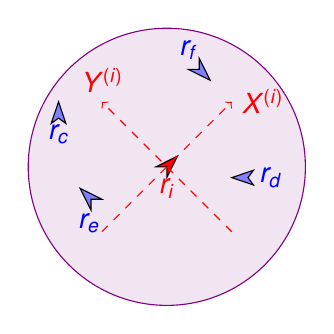
\begin{tikzpicture}[scale=0.55]
            \draw[violet, fill=violet!10] (3, 3) circle (3.2);
            \draw[fill=red] (3,3) -- (2.75,3) -- (3.25,3.25) -- (3,2.75)   	-- cycle;
            \node[color=red] at (3, 2.5) {$r_i$};
            
            \draw[color=red, dashed, ->] (1.5,1.5) -- (4.5,4.5) node[right] {$X^{(i)}$};
            \draw[color=red, dashed, ->] (4.5,1.5) -- (1.5,4.5) node[above] {$Y^{(i)}$};
            
            \draw[fill=blue!50] (0.5,4.5) -- (0.33,4) -- (0.5,4.125) -- (0.67,4) 	-- cycle;
            \node[color=blue] at (0.5,3.75) {$r_c$};
            \draw[fill=blue!50] (4,5) -- (3.75,5.5) -- (3.75,5.25) -- (3.5,5.25)   	-- cycle;
            \node[color=blue] at (3.5,5.7) {$r_f$};
            \draw[fill=blue!50] (1,2.5) -- (1.25,2) -- (1.25,2.25) -- (1.5,2.25)   	-- cycle;
            \node[color=blue] at (1.2,1.7) {$r_e$};
            \draw[fill=blue!50] (5,2.92) -- (4.5,2.75) -- (5,2.58) -- (4.875,2.75)  -- cycle;
            \node[color=blue] at (5.4,2.75) {$r_d$};
            % \draw[fill=blue!50] (-0.5,2.5) -- (-0.5,2.75) -- (-0.75,2.25) -- (-0.25,2.5)  -- cycle;
            % \node[color=blue] at (-0.75,3) {$r_b$};
          \end{tikzpicture}
          \caption{Robot $r_i$ and its neighbors $r_c, r_d, r_e,
            r_f$ in its local $X^{(i)}$-$Y^{(i)}$ coordinates. The
            disk describes $r_i$'s range.}
          \label{fig:robotmodel}
        \end{figure}
      \end{column}%
    \end{columns}
\end{block}
\end{frame}
%%%%%%%%%%%%%%%%

\section{Lattice Graph}
% definition of lattice graph
\begin{frame}{Lattice Graph}
  \begin{block}{}
    \begin{bclogo}[couleur=orange!10, arrondi=0.2, ombre=true]{Definition}
      A \textbf{lattice graph} is a strongly connected directed
      multigraph in which each edge $e$ is labeled with a rigid body
      transformation $T(e)$ and each $\edge{v}{T(e)}{w}$ has an
      inverse edge $\edge{w}{T(e)^{-1}}{v}$.  
    \end{bclogo}
    \begin{bclogo}[couleur=orange!10, arrondi=0.2, ombre=true]{} 
      Given a lattice graph $G=(V, E)$ and a set of robots $R = \{
      r_1, \ldots, r_n \}$, we say that $R$ \textbf{satisfies} $G$ if
      there exists a role function $f: R \rightarrow V$ that preserves
      the neighborhood structure of $G$.
      % 
      Specifically, for any $i$ and $j$, if $r_i$ and $r_j$ are neighbors, 
      there must exist an edge
      $e_{ij}: \edge{f(r_i)}{}{f(r_j)}$ in $E$, such that
      $$ T(r_j) = T(r_i) T(e_{ij})$$
    \end{bclogo}
  \end{block}
\end{frame}

\begin{frame}{Lattice Graph}
  \begin{block}{}
   
  \end{block}
\end{frame}

\subsection{Robot Authority}
% installation on GNU/Linux
\begin{frame}{Authority}
  \begin{block}{}
    \begin{bclogo}[couleur=orange!10, arrondi=0.2, ombre=true]{Definition} 
      An \textbf{authority} is an ordered list of robot IDs
      $$ \langle \id_1, \ldots, \id_k \rangle $$
      The first ID in the list, $\id_1$ is called the \textbf{root} ID.
      Likewise, the final ID in the list, $\id_k$ is called the
      \textbf{sender} ID.  The number $k$ of IDs in the list is called
      its \textbf{length}.
    \end{bclogo}
  \end{block}
\end{frame}
%%%%%%%%%%%%%%%%
% help me iron out the bugs or give me some comment and suggestions
\begin{frame}{Construct Authority Tree}{}
  \begin{itemize}
    \item<1-> There are probably still some bugs in the theme. If you should find one, then please let me know. No bug is too small!
    \item<2-> Also, please contact me, if you have some exciting new ideas or just some simple usability improvements.
  \end{itemize}
\end{frame}
%%%%%%%%%%%%%%%%


\subsection{Algorithm}
% installation on Microsoft Windows
\begin{frame}{Algorithm}{}
  \begin{block}{Windows with MiKTeX}
    Apparently, MiKTeX does not include a local latex directory tree by default. Therefore, you first have to create it.
    \begin{enumerate}
      \item To do this, create a folder {\tt <somewhere>} named, e.g., {\tt texmf}
      \item Add this folder in the Roots tab of the MiKTeX Settings dialog
      \item Place the {\tt <dirstruct>} in your newly created local latex directory tree\\
    {\tt <somewhere>\textbackslash texmf}\\
      \item Open the MiKTeX Settings dialog and click Refresh FNDB.
    \end{enumerate}
  \end{block}
\end{frame}
%%%%%%%%%%%%%%%%

% installation on Microsoft Windows Cont'd
\begin{frame}{Local Task Assignment}{}
  \begin{block}{Windows with TeX Live}
    In the advanced TeX Live Installer, you can manually change the default position of the root of the local latex directory tree. However, we assume the default position below.
    \begin{enumerate}
      \item Place the {\tt <dirstruct>} in your local latex directory tree\\
        {\tt \%USERPROFILE\%\textbackslash texmf}\\
        If it does not exist, create it. In XP {\tt \%USERPROFILE\%} is\\
      {\tt c:\textbackslash Document and Settings\textbackslash<username>}\\
      by default, and in Vista and above it is by default\\
      {\tt c:\textbackslash Users\textbackslash<username>}
      \item Open the TeX Live Manager dialog and select 'Update filename database' under 'Actions'.
    \end{enumerate}
  \end{block}
\end{frame}
%%%%%%%%%%%%%%%%

\subsection{Robot Motion Control}
% text
\begin{frame}{Installation}{Mac OS X}
  \begin{block}{Mac OS X with MacTeX}
     Place the {\tt <dirstruct>} in the root of your local latex directory tree. By default it is\\
        {\tt \textasciitilde /Library/texmf}\\
        If the root does not exist, create it. The symbol {\tt \textasciitilde} refers to your home folder, i.e., {\tt /home/<username>}
  \end{block}
\end{frame}
%%%%%%%%%%%%%%%%

% list of required packages
\begin{frame}{Installation}{Required Packages}
  Of course, you have to have the Beamer class installed. In addition, the theme loads two packages
  \begin{itemize}
    \item TikZ\footnote{By the way, TikZ is an awesome package for creating beautiful graphics. If you do not believe me, then have a look at these \chref{http://www.texample.net/tikz/examples/}{online examples} or the \chref{http://tug.ctan.org/tex-archive/graphics/pgf/base/doc/generic/pgf/pgfmanual.pdf}{pgf user manual}. If you want to create beautiful plots, you should use the pgfplots package which is based on TikZ.}
    \item calc
  \end{itemize}
  These packages are very common and should therefore be included in your latex distribution.
\end{frame}
%%%%%%%%%%%%%%%%

\section{Results}
\subsection{Experiments}
% list of the themes and options
\begin{frame}{User Interface}{Loading the Theme and Theme Options}
  \begin{block}{The Presentation Theme}
    It is very simple to load the presentation theme. Just type\\
    {\tt \textbackslash usetheme[<options>]\{AAUsimple\}}\\
    which is exactly the same way other beamer presentation themes are loaded. The presentation theme loads the inner, outer and color AAU Simple theme files and passes the {\tt <options>} on to these files.
  \end{block}
  \begin{block}{The Inner Theme}
    You can load the inner theme directly by\\
    {\tt \textbackslash useinnertheme\{AAUsimple\}}\\
    and it has no options.
  \end{block}
\end{frame}
%%%%%%%%%%%%%%%%

% list of the themes and options
\begin{frame}{User Interface}{Loading the Theme and Theme Options}
  \begin{block}{The Outer Theme}
    You can load the outer theme directly by\\
    {\tt \textbackslash useoutertheme[<options>]\{AAUsimple\}}\\
    Currently, the theme option is
  \begin{itemize}
    \item {\tt shownavsym}: show the navigation symbols
  \end{itemize}
  \end{block}
\end{frame}
%%%%%%%%%%%%%%%%

% list of the themes and options
\begin{frame}{User Interface}{Loading the Theme and Theme Options}
  \begin{block}{The Color Theme}
    You can load the color theme directly by\\
    {\tt \textbackslash usecolortheme\{AAUsimple\}}\\
    and it has no options.
  \end{block}
  \pause
  \begin{block}{The Color Element {\tt AAUsimple}}
    The color theme defines a new beamer color element named {\tt AAUsimple} whose foreground and background colors are
    \begin{itemize}
      \item fg: {\usebeamercolor[fg]{AAUsimple}light blue (\{RGB\}\{194,193,204\})}
      \item bg: {\usebeamercolor[bg]{AAUsimple}dark blue (\{RGB\}\{33,26,82\})}
    \end{itemize}
    You can use these colors in the standard beamer way by using the command
    {\tt \textbackslash usebeamercolor[<fg or bg>]\{AAUsimple\}}. See the beamer manual for instructions.\\
 \pause Note that this version of the theme is an official AAU version and is in accordance with the \chref{http://aau.designguides.dk/}{AAU design guide}. However, you can easily change it (including the colour of the logo) by following the steps in {\tt beamercolorthemeAAUsimple.sty}.
  \end{block}
\end{frame}
%%%%%%%%%%%%%%%%

\subsection{Results}
% how to modify the theme
{\setbeamercolor{AAUsimple}{fg=gray!50,bg=orange!50}
 \setbeamercolor{structure}{fg=red}
 \setbeamercolor{frametitle}{use=structure,fg=structure.fg}
 \setbeamercolor{normal text}{bg=gray!20}
\begin{frame}{User Interface}{Modifying the Theme}
  \begin{itemize}
    \item<1-> The default configuration of fonts, colors, and layout complies with the \chref{http://aau.designguides.dk}{AAU design guidelines} and is the \alert{official} version of the theme.
    \item<2-> However, you can modify specific elements of the theme through the templates provided by the beamer class. Please refer to the beamer user manual for instructions.
    \item<3-> For example, on this slide the following commands have been used
  \end{itemize}
\end{frame}}
%%%%%%%%%%%%%%%%

\subsection{Conclusions}
% Widescreen Support
\begin{frame}{Conclusions}{}
\begin{block}{}
   \begin{itemize}
        \item Change the header colours:\\
        {\tt \textbackslash setbeamercolor\{AAUsimple\}\{fg=blue!20,bg=red!50\}}
        \item Change the color of the structural elements:\\
        {\tt \textbackslash setbeamercolor\{structure\}\{fg=black\}}\\
        \item Change the frame title text color:
        {\tt \textbackslash setbeamercolor\{frametitle\}\{use=structure, fg=structure.fg\}}
        \item Change the background color of the text
        {\tt \textbackslash setbeamercolor\{normal text\}\{bg=gray!20\}}
      \end{itemize}
\end{block}
\end{frame}
%%%%%%%%%%%%%%%%


\section{Feedback}
%\subsection{Known Problems}
%% known problems
%\begin{frame}{Feedback}{Known Problems}
%  \begin{description}
%    \item[Overlapping footnote] You might have problems with a too wide footnote text width. This is problem with older versions of Beamer, and it can be resolved by updating Beamer to a newer version. You can read more about it in \chref{https://bitbucket.org/rivanvx/beamer/issue/200/width-of-footnote-in-a-sidebar-theme}{this bugreport}.
%  \end{description}
%\end{frame}
%%%%%%%%%%%%%%%%%

\subsection{Contact Information}
% contact information
\begin{frame}{Questions}{}
In case you have any comments, suggestions or have found a bug, please do not hesitate to contact me. You can find my contact details below.
  \begin{center}
    {\LARGE THANK YOU!}
  \end{center}
\end{frame}
%%%%%%%%%%%%%%%%

\end{document}
